\documentclass{sig-alternate-ipsn13}

\usepackage{comment}
\usepackage{times}
\usepackage{epsfig}
\usepackage{psfrag}
\usepackage{subfigure}
\usepackage{graphicx}
\usepackage{amssymb}
\usepackage{amsmath}
\usepackage{mathenv}
\usepackage{epstopdf}
\usepackage{fancyhdr}
\usepackage[ruled,algonl]{algorithm2e}  % for snazzy algorithm package
\usepackage{mathrsfs,bbm}

\begin{document}

\title{Early Congestion Notification For Cyber-Physical Smart Grid Nodes. 
\thanks{This work was supported in part by the Future Renewable
Electric Energy Delivery and Management Center, a National Science Foundation
supported Engineering Research Center under grant NSF EEC-081212}}

\author{
\alignauthor
Ashish Choudhari, Harini Ramaprasad \\
       \affaddr{\em Department of Electrical and Computer Engineering,}\\
       \affaddr{\em Southern Illinois University Carbondale} \\
\and
\alignauthor
Bruce McMillin, Sriram Chellappan \\
       \affaddr{\em Department of Computer Science,}\\
       \affaddr{\em Missouri University of Science and Technology}
}

\maketitle

\begin{abstract}
\label{sec:abstract}

Cyber-Physical Systems (CPS) consist of computational components interconnected by computer networks that monitor and control switched physical entities interconnected by physical infrastructures. To ensure a tight integration among the components in CPS we employ a novel approach that composes the correctness of components instead of their functionality using conjunction of non-interfering logical invariants. Our distributed algorithm developed for smart power grid nodes uses this approach to adaptively schedule power migrations in such a way that the stability of both the computer network and the physical system are maintained. In this paper we mainly focus on network congestion and explore a well known Explicit Congestion Notification (ECN) scheme from CPS context and demonstrate the significant improvement in overall CPS efficiency and stability. Experimentation results show how the power transfers between smart grid nodes are unaffected if nodes are allowed to exploit ECN scheme while also taking necessary actions to reduce network congestion.
\end{abstract}
\section{Introduction}
\label{sec:introduction}

Smart Power Grid~\cite{huang11} is a prime example of Cyber-Physical System 
(CPS) where the goal is to have embedded computing devices monitor and control 
distributed generation, storage and transfer of power in a safe, reliable, 
efficient and secure manner. Ensuring stability and correctness (both logical and temporal)
of the system as a whole is a major challenge in CPS design. Any incorrectness or 
instability in one component can impact the same features of other components. 
For example, an action in the physical domain could affect the network domain and 
vice-versa, thus making correct scheduling of these actions paramount to overall system
stability. The fundamental challenge in developing a design framework that
unifies the various components is the heterogeneity of the component types,
resulting in semantic gaps that must be bridged. 

% comparison
Existing papers largely consider the stability of one or two components in
isolation. For example, network delays affect system stability and considerable
work focusses on determining system stability bounds as a function of injected
delay~\cite{hespanha07}. Results from switched-systems theory~\cite{donkers11}
model the stability of the plant. Hybrid automata~\cite{henzinger96} and timed
I/O automata~\cite{alur94} represent a simultaneous mix of continuous and
discrete states in the verification process~\cite{chutinan03,tomlin03}.
Real-time scheduling is traditionally a function of \emph{a priori} time
bounds~\cite{liu00}. To consider components individually, or in pairs, requires
that they be very stable such that the composition of the components into a CPS
is stable.

In our work, we employ a fundamentally different approach that composes
correctness instead of functionality. The basic idea, depicted in
Figure~\ref{fig:invariant_conjunction}, is to express the stability and
correctness constraints of all components in the form of logical {\em invariants} 
and ensure that system actions are performed only if and when they are guaranteed not 
to violate the conjunction of these invariants. This approach is not only limited
to smart power grid design but can also be generalized to different cyber-physical systems 
with different functionalities. 

\begin{figure}[htb]
  \begin{center}
%    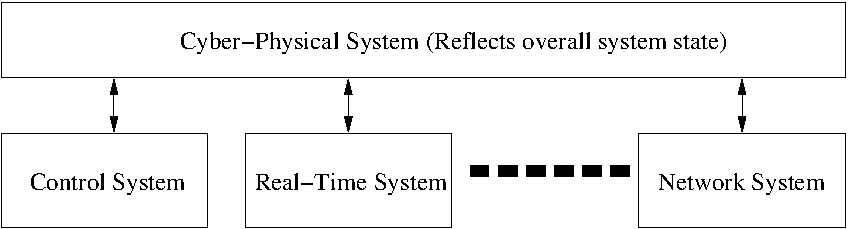
\includegraphics[width=0.45\textwidth]{Figures/cps-n-domains.pdf}
     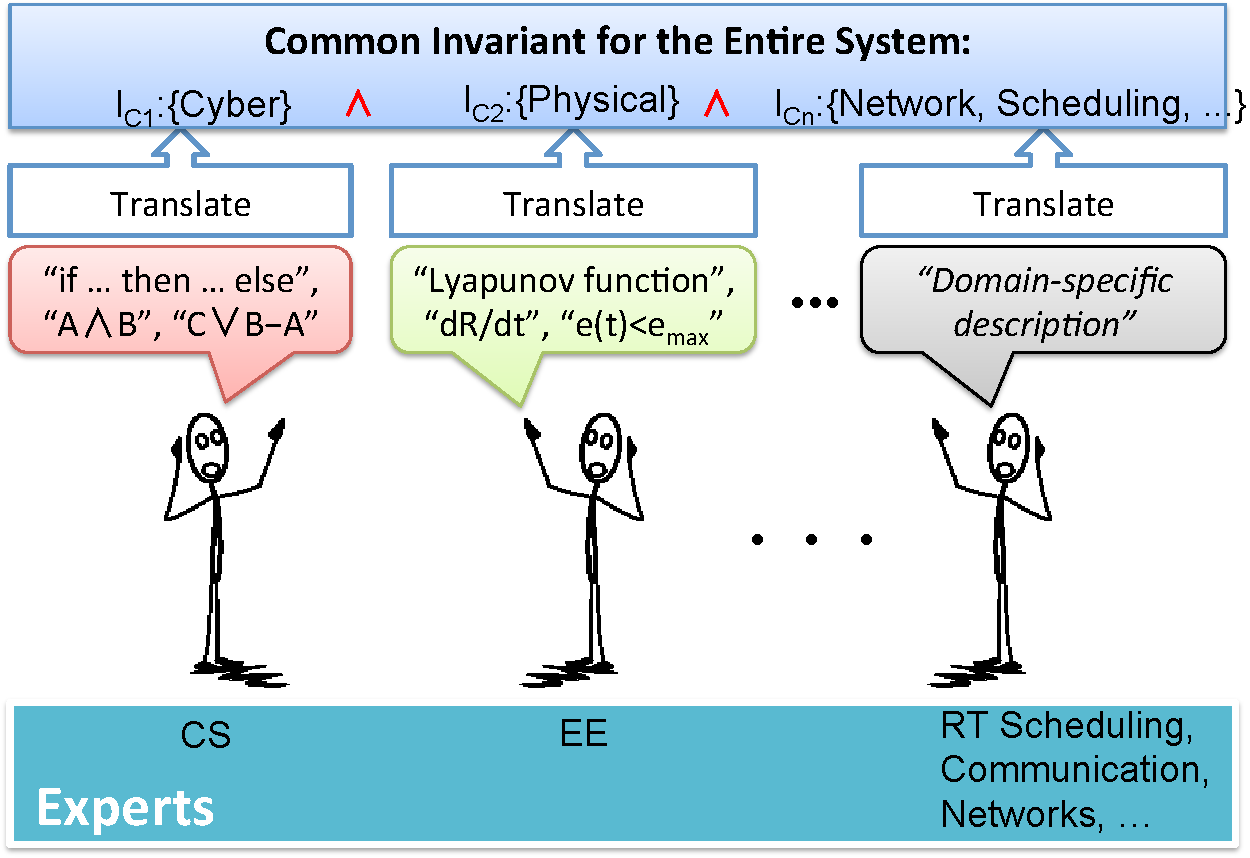
\includegraphics[width=0.9\columnwidth]{Figures/Invariant_Overview.pdf}
  \caption{Overview of invariant-based approach}
  \label{fig:invariant_conjunction}
  \end{center}
\end{figure}

The state of the physical system and, hence, its stability, is dependent on
power transfers (series of power migrations) initiated by the cyber algorithm
within each node in the system and by the state of the communication network
that carries messages between the cyber nodes to signal initiation and
acknowledgement of physical power migrations. The state and stability of the
communication network is in turn affected by the number of migration messages in
transit at any given time. In recent work[*****cite COMPSAC], we developed a 
scheduling invariant for our distributed, adaptive algorithm for scheduling power 
migrations between nodes in a smart grid and demonstrate that conjunction of such a
scheduling invariant and an invariant for physical system state is necessary to 
maintain overall system stability. In contrast to traditional real-time scheduling, 
{\em correct} scheduling in our context refers to initiating actions at appropriate 
times in a way that system stability is maintained rather than insisting that every 
action is initiated at a pre-defined time and must adhere to a pre-defined deadline. 
In order to improve efficiency along with stability, components in CPS must have 
certain amount of inter-component information. In the current paper, we focus on 
improving the efficiency while also maintaining the stability of smart grid nodes 
by exploiting the network congestion information obtained from Early Congestion 
Notification (ECN) scheme, wherein packets are marked indicating impending congestion,
instead of dropping them\cite{floyd1994tcp, ramakrishnan1999proposal, 
ramakrishnan2001addition}. We allow the smart grid nodes to sense the possible 
upcoming network congestion and change the amount of power being transferred with 
every power migrate message in order to compensate for reduced rate of power transfers.
As of our knowledge, this is the first work that explore ECN scheme from CPS context
for the benefit of physical system efficiency as well as take necessary action to 
reduce network congestion.

The rest of this paper is organized as follows. Section \ref{sec:related_work}
provides some background information and discusses related work. We present our
system model and assumptions in Section \ref{sec:assumptions}. Section
\ref{sec:invariants} presents our physical system 
invariant and adaptive scheduling invariant. Section \ref{sec:power_management_algo} 
presents our resulting power management algorithm. Our simulation setup is introduced 
in Section \ref{sec:simulation_setup} and results are presented in Section
\ref{sec:results}. Section \ref{sec:discussion} presents a brief discussion and
conclusions are presented in Section \ref{sec:conclusions}.


\section{Background and Related Work}
\label{sec:related_work}

Most of the Cyber-physical systems are switched, continuous time dynamic systems with changes occurring at discrete time intervals~\cite{liberzon03}. Analyzing CPS is a complicated task, as it consists of tight coupling of various components that are heterogeneous in nature, such as, cyber,  physical and network. In CPS, actions performed in one component should not affect the stability in another components. Therefore, it is mandatory to schedule \textit{correct} actions at \textit{correct} time in each component of CPS in order to maintain overall system stability. However, only stability and correct scheduling is not enough, the system should also be adaptive in nature when uncertain components are present in the composed CPS. Typically, most of the CPS kind of applications, involve communication network as one of the important components ("smart grid" as a prime example). Standalone physical systems with computational capability, such as power plants, vehicular systems, medical devices, and robotics - just to name few - have been deeply studied in the literature, but when these kind of systems are interconnected through unreliable or uncertain communication network, like internet, physical system aspects, assumptions, control strategies and functional behavior is affected due to the unpredictability of transmission time in the communication network. 

A verification technique for Cyber-Physical systems was recently proposed in~\cite{DAC_2012_CPS_verification} assuming communication network to be CAN, FlexRay. etc, wherein authors use structured properties of network infrastructures and efficiently bound network delays. 
In~\cite{SmartGridLoadScheduling}, authors propose an idea of scheduling power demands for optimal energy management in smart-grid, but they do not consider the network behavior. In traditional real-time systems, dynamic adaptation is normally performed at "sporadic intervals" using elastic scheduling techniques~\cite{Buttazzo_IEEE_Jornl_2002} and feedback scheduling~\cite{FeedbackScheduling07}, but CPS requires continuous adaptation. Adaptive scheduling proposed in ~\cite{AdaptiveScheduling_DASC_1999}, dynamically changes the task execution rate based on the observed system behavior, but requires complete abstraction of physical and network parameters. Similar approach can be taken to dynamically change the power transfer rate across the smart-grid nodes based on the observed network conditions, but abstraction of internet like network parameters (eg. RTT, Round-Trip time) is non-trivial. In our recent paper~\cite{acsmartgrid}, we proposed an adaptive algorithm which schedules power migrate messages between CPS smart-grid nodes based on the observed round-trip times in internet like network. This algorithm forms invariant which in conjunction with physical system invariant achieves stability of the overall system. The main reason of unpredictable round-trip times (in internet) is the nature of the traffic, increase in traffic might lead to exponential increase in transmission delays and can also cause messages to drop.

[******add citations]
{\bf Protocols for CPS,} although internet protocols such as TCP are well known for reliability, TCP relies on packet drops caused due to overflow of queues at gateways as an indication of network congestion. 
In smart grid context, every message is responsible for a small amount of power in the
grid, therefore a loss of message is directly associated to the grid stability. TCP by controlling 
its transmission rate can effectively reduce packet drops if transport is capable of ECN.
But, congestion information obtained from network is completely hidden from the application
running over TCP. In order to know ECN in application, User Datagram Protocol (UDP) is a perfect choice.
It is then application's responsibility to adapt according to network conditions and take 
necessary actions upon detection of congestion in the network.
[******end citations]


\section{System Model And Assumptions}
\label{sec:assumptions}

{\bf Power Management Architecture.} Figure~\ref{fig:SmartGridArchi-fig} shows
the architecture of a future generation smart grid (SmartGrid)~\cite{huang11}.
The system is essentially a microgrid consisting of energy storage devices
(DESD), energy resources (DRER) and LOADs. Each node is potentially owned and
located in a residence or business and the basic idea is to share power among
nodes in order to benefit the overall system. Intelligent flow controllers
(nodes) contain Solid State Transformers (SSTs), that are physical actuators
controlling power flow to and from a shared electrical bus under the direction
of co-operating Distributed Grid Intelligence (DGI) processes.

The DGI processes are cyber algorithms that choose, negotiate and manage power
transfers among nodes based on local information and information about the
states of other nodes that is periodically exchanged among nodes. In the current
work, we assume that all nodes are synchronized, for the sake of simplicity.
Nodes periodically exchange state information with each other in a state
collection phase. Next, a negotiation phase is performed in which nodes conduct
negotiations to identify which power transfers need to be performed among nodes.
The identified power transfers between pairs of nodes are then performed in a
power transfer phase. One cycle is depicted in Figure\ref{fig:cycle}, with one
or more negotiation and power transfer phase pairs after a state collection
phase. This entire cycle of state collection, negotiation and power transfer
phases is repeated.

\begin{figure}[htb]
  \begin{center}
    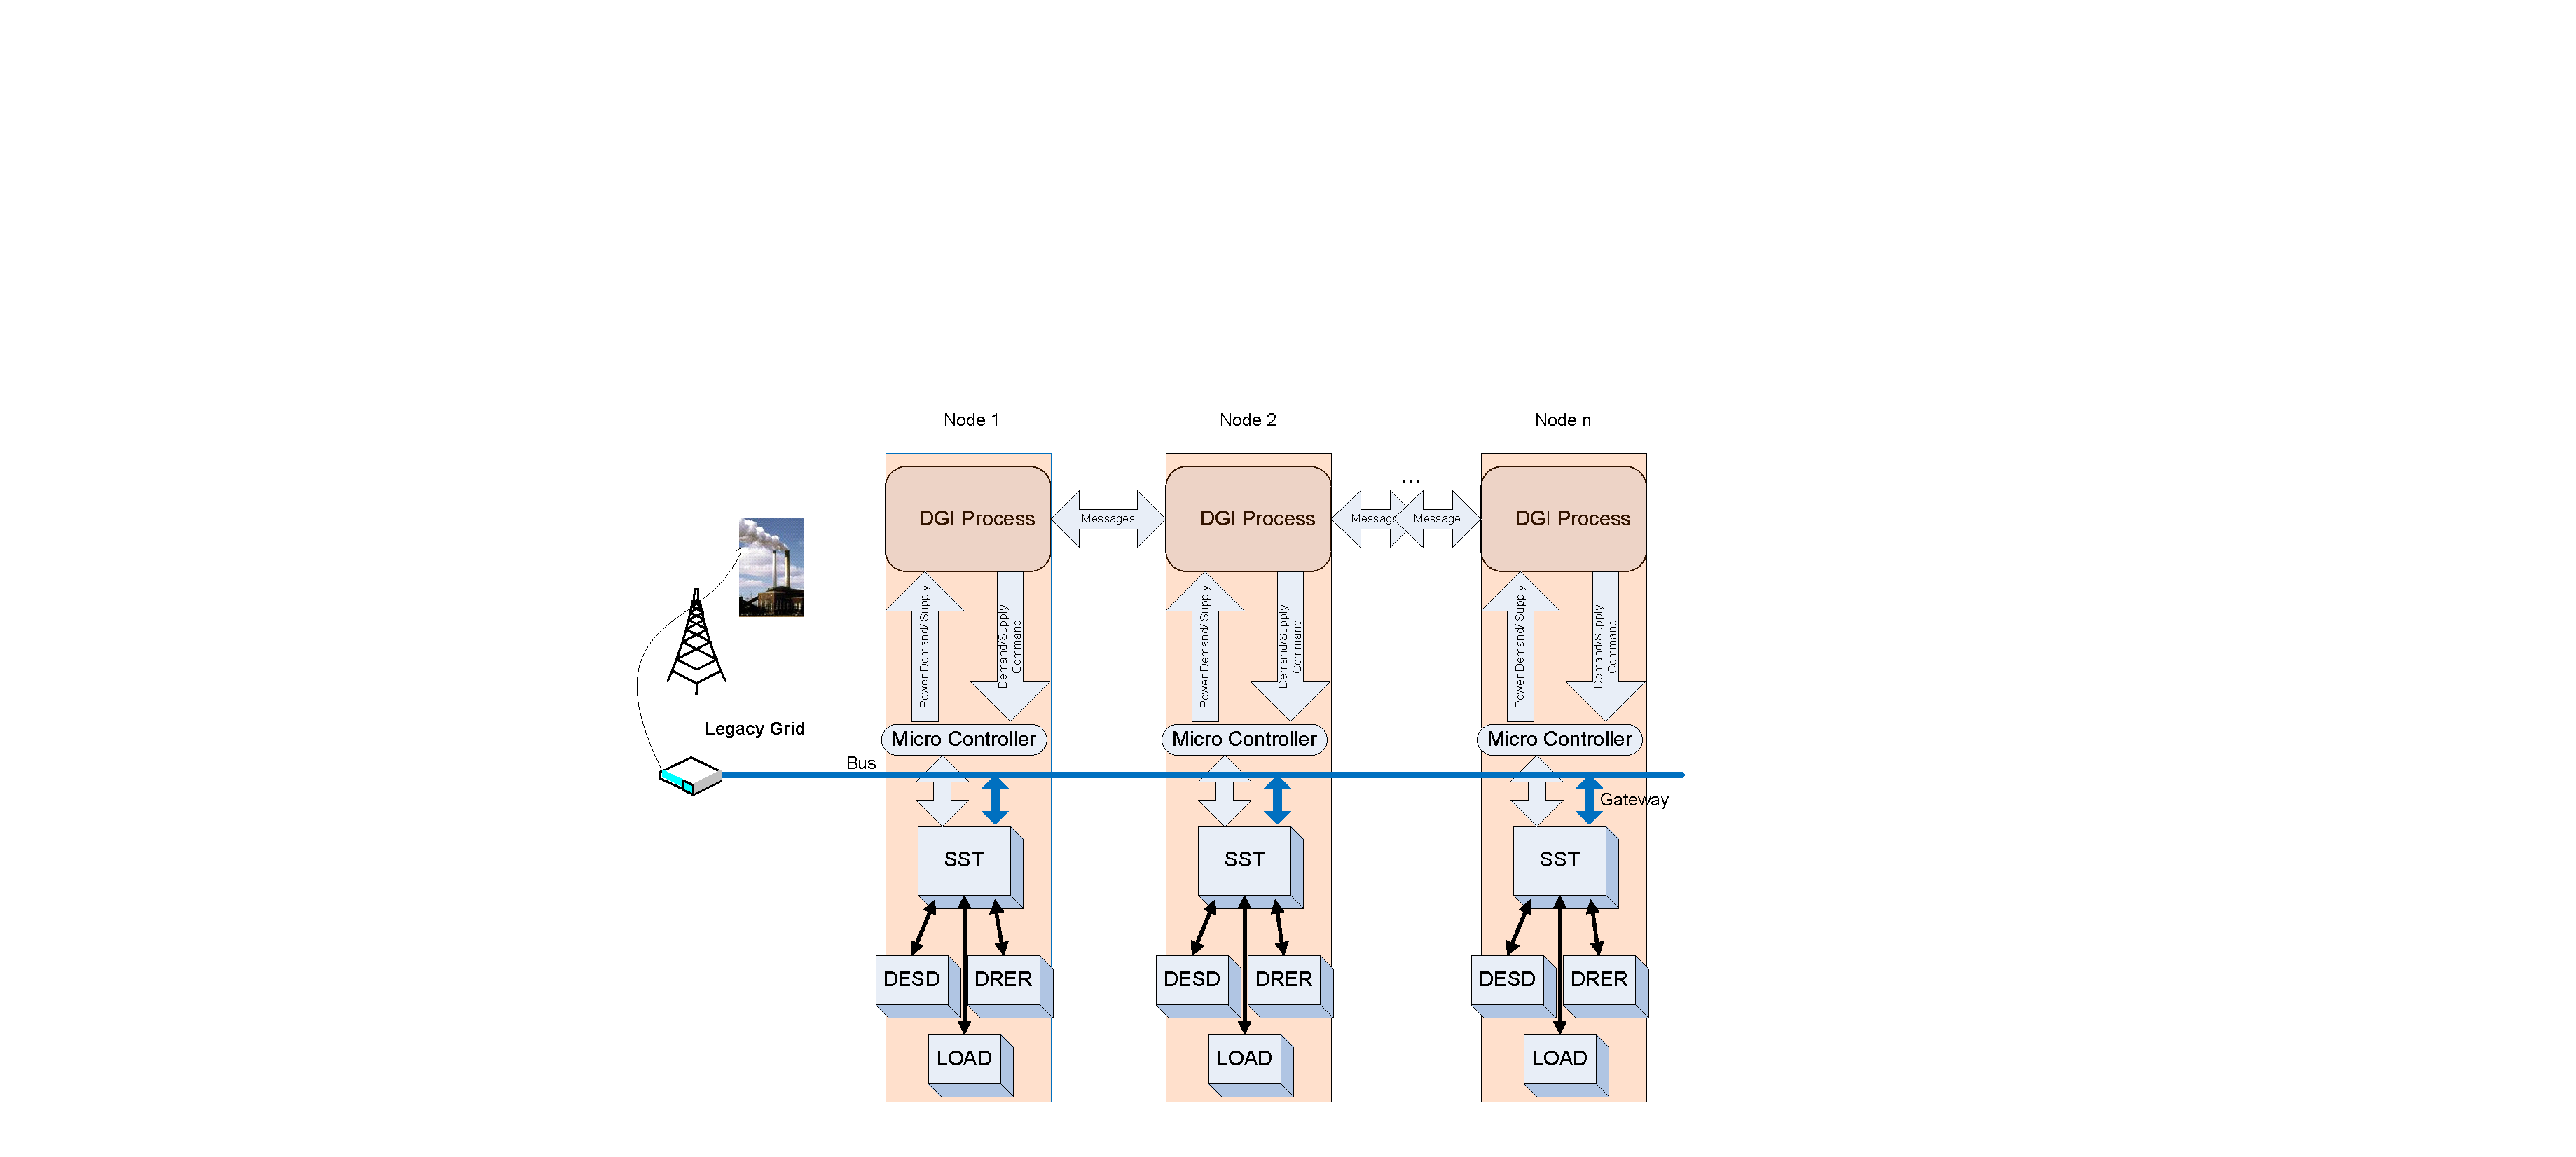
\includegraphics[width=0.45\textwidth]{Figures/DistributedLoadBalancing3.pdf}
  \caption{Smart Grid Power Management Architecture}
  \label{fig:SmartGridArchi-fig}
  \end{center}
\end{figure}

\begin{figure}[htb]
  \begin{center}
    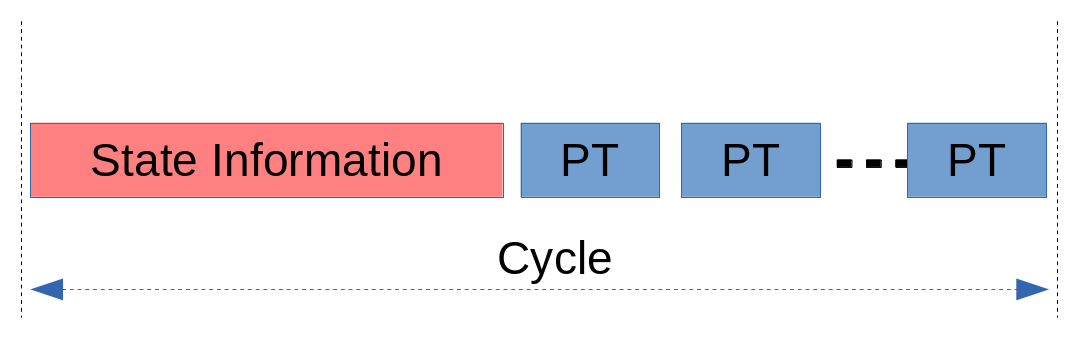
\includegraphics[width=0.45\textwidth]{Figures/cycle_fig.png}
  \caption{A single cycle of collecting state information followed by many negotiation and power transfer phases (PT)}
  \label{fig:cycle}
  \end{center}
\end{figure}

{\bf Power Transfer Model.} Power transfers within one phase are performed as a
series of (periodic) power migrations, each transferring a given quantum (say
$\delta$) of power. The cyber algorithm on the source (sender) node sends
appropriate control signals to the local physical actuators to add a quantum of
power to the electrical bus and sends a power migration message to the
destination (receiver) node signaling this. Upon receiving this power migration
message, the destination node sends control signals to its local physical
actuators to remove a quantum of power from the electrical bus and sends an
acknowledgement message to the source node.

{\bf Physical System Model.} The physical system is a finite inertia microgrid,
that is, a power system with a small number of generators and loads that acts
independently of the grid. There is a relatively small rotating generator,
whose inertia dominates the dynamics as described in the next section. There
are some number of controllable nodes that participate in the power management
by acting as either loads or generators. Nodes with excess generating capacity
transfer power to nodes that have excess load.

{\bf Communication Model.} 
Each node in the network runs an adaptive message scheduling algorithm that schedules power migrate messages in any given 
topology, based on the observed communication latencies at a given node. 

%\section{System Analysis And Invariant Formation}
%\label{sec:invariants}
%
%\subsection{Physical System Analysis}
%The physical system must satisfy one out of several criteria in order to be
%stable. The criteria are derived from an analysis of the continuous-time
%dynamics of the system, which are modeled as
%\begin{eqnarray}
%  \frac{d\omega}{dt} &=& -\frac{V_1 V_2}{J \omega X}sin(\theta - \theta_0)-\frac{D}{J}(\omega - \omega_0) + \frac{P_{imb}}{J\omega} - \frac{kP^2}{J\omega}, \nonumber \\
%  \frac{d\theta}{dt} &=& \omega - \omega_0,
%  \label{eqn:swing1}
%\end{eqnarray}
%where $\omega$ is the frequency, $\theta$ is the phase angle of the generator voltage, $\omega_0$ and $\theta_0$ are their nominal
%values, $P_{imb}$ is the net power imbalance due to outstanding messages,
%and the other terms are various physical parameters.  The error energy, given by
%\begin{equation}
%  V(\omega, \theta) = \frac{J}{2} (\omega - \omega_0)^2 + \frac{V_1 V_2}{\omega X}(1-cos(\theta - \theta_0)).
%  \label{eqn:lyap}
%\end{equation}
%is a Lyapunov function (that is, a positive-definite function with a
%non-positive time derivative) if the system satisfies $I_{P1}$, given by
%\begin{equation}
%\left\{
%\begin{matrix}
%I_{P1}: (\omega - \omega_0)^2 \left(D\omega + m \right) \\ + (\omega - \omega_0)(kP^2)  > \delta K (\omega - \omega_0)
%\end{matrix}
%\right\}
%\label{eqn:grid4}
%\end{equation}
%With other factors, $I_{P1}$ ultimately imposes a limit on $\delta * K$, where
%$\delta$ is the quantum of power migrated with each message and $K$ is the
%number of outstanding messages.
%
%In general, if a Lyapunov function exists for a particular physical system, then
%the system is stable. However, there are other conditions that also ensure
%stability for a switched system, which is a continuous-time system that is
%subject to external switching events. A \emph{Lyapunov-like} function
%\cite{branicky98,ye98impulse,ye98hybrid} is similar to a Lyapunov function in
%that it must be positive-definite, but its value may increase under some
%conditions. If the value of the Lyapunov-like function decreases at each
%switching event, then the system is stable. A final option is that the error may
%not decay to zero, but is bounded.
%
%{\bf Physical System Invariant($I_P$).}
%Combining the three conditions, a single invariant may be found,
%\begin{equation}
%  \{I_P : I_{P1} \lor (V(\omega, \theta) < V_{bound}) \lor (V(t) \leq V(t_{x}))\}
%  \label{eqn:IP}
%\end{equation}
%where $V_{bound}$ is the maximum allowable value of $V$, $V(t)$ is the value of
%$V(\omega, \theta)$ at the present time and $V(t_{x})$ is its value at the most
%recent previous violation of $I_{P1}$ due to a large value of $K$. Prior work
%\cite{paul2011,paul12thesis} has demonstrated that the system can be stable for 
%certain combinations of steady-state power imbalance and droop constants in 
%the SST controllers.
 
\section{Adaptive Communication} 
\label{adap_comm}

Physical system stability at any point of time is determined by the product of power migrate messages
$K$ in transit and amount of power $\delta$ transferred with every message. 
Stability of network depends only on $K$, where $K$ is a function of rate(s) of power migration
and observed round-trip time between source and receiver nodes in the communication network.
To provide safe and stable operation, an upper bound $Kmax_{global}$ for maximum outstanding messages 
is established prior to power transfer phase, based on physical and network restrictions. $Kmax_{global}$ 
is then distributed as in Figure~\ref{fig:Kmax_distribution} among the nodes that have excess power 
and needs to undergo power migrations. For example, in Equation~\ref{eq:kmax_distrib}, $Kmax_{global}$ 
is distributed among $n$ nodes in proportion to excess power. After distribution, each excess power 
node has a limit $Kmax_s$ on maximum number of outstanding messages it can have in the network at any 
point of time.

\begin{equation}
Kmax_s = \lfloor(\frac{P_s}{\sum_{i=1}^{n} P_i}) * Kmax_{global}\rfloor
\label{eq:kmax_distrib}
\end{equation}

\begin{figure}[htb]
  \begin{center}
    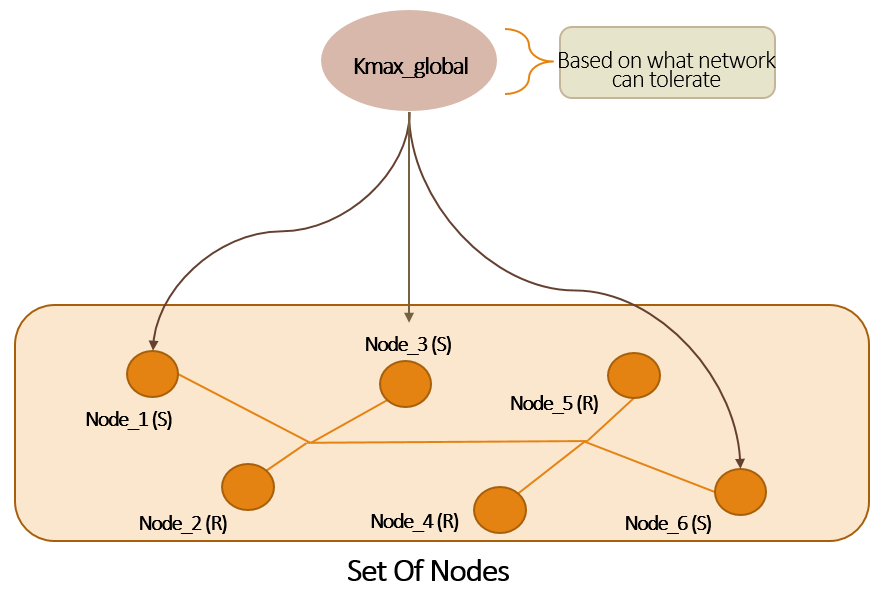
\includegraphics[width=0.45\textwidth]{Figures/kmax_distri.png}
  \caption{$Kmax_{global}$ Distribution Among Sender Nodes}
  \label{fig:Kmax_distribution}
  \end{center}
\end{figure}

The message scheduling algorithm running at node $s$, adapts the power message migration 
rate $r_s$ or, inversely, the period $p_s$ such that the number of outstanding messages
of node $s$ at any given time, never exceeds its maximum allowed outstanding messages $Kmax_s$.


\subsection{Scheduling Algorithm}
\label{sec:sched_algo_explanation} 


Every power migrate message initiated by node $s$ is assigned a relative deadline $D_s$ determined 
from the current expected response time ($RT_s^{ex}$). Where, $RT_s^{ex}$ is the average of certain number 
of previously observed response times (response time also known as round-trip time). 

If an acknowledgment $m_a$ of message $m$ is not received before its deadline (\textit{deadline miss}) 
indicates that there is a possibility of congestion in the network. 

Therefore, in an effort to reduce congestion, the algorithm increases its expected response time $RT_s^{ex}$
by a pre-defined margin ($RTMargin$) and determines a smaller transmission rate and a larger relative deadline.

In the worst case, power migration will only be done if acknowledgments for all the outstanding messages is received. 

Whereas, if certain $CtrMax$ (response time counter limit) number of acknowledgments are received 
consecutively with smaller response times than expected, then the algorithm increases its transmission rate 
and calculates a more tighter (smaller) relative deadline, ensuring that physical and network stability is 
still maintained. Note that $RTMargin$ and $CtrMax$ are configurable system parameters and are assumed to 
be constant for all nodes in a given power transfer phase. 


Following is the list of events which sets the scheduling algorithm in motion.\\
\\*1. Initialize Event.
\\*2. Sent power message event.		
\\*3. Ack received event.
\\*\- 3.1. Ack received is better event.
\\*\- 3.2. Ack received after deadline miss event.
\\*4. Deadline miss event.
\\*5. Receive power event.


{\bf Message Scheduling Invariant ($I_S$).}

For a given power transfer phase and based on above $Kmax_s$, $p_s$ constraints, following scheduling invariant
$I_s$ can be formed, shown in
Equations \ref{eq:sched_invariant_1} - \ref{eq:sched_invariant_4}.
\begin{equation}
\{I_S = I_k \wedge I_c \wedge I_p\}
\label{eq:sched_invariant_1} 
\end{equation}
\begin{equation}
I_k: K_s < Kmax_s 
\label{eq:sched_invariant_2}
\end{equation}
\begin{equation}
I_c: RT_s^{ex} \leq PT - t 
\label{eq:sched_invariant_3}
\end{equation}
\begin{equation}
I_p: t - LT(s) \geq p_s
\label{eq:sched_invariant_4}
\end{equation}

Here, $PT$ is the end time of the power transfer phase, $t$ is the time at which
the invariant is evaluated and $LT(s)$ is the time at which the last power
migration message was initiated by node $s$. Work done in~\cite{acsmartgrid} shows the importance of
composing system correctness through conjunction of physical $I_p$ and scheduling $I_s$ invariants in order
to maintain system stability.






\section{Adaptive Scheduling with Early Congestion Notification}
\label{sec:adaptive_with_ecn}

In this section, we propose modifications required for adaptive power scheduling algorithm~\cite{acsmartgrid} to support Early Congestion Notification (ECN) obtained from the ECN capable transport. We explain ECN mechanism in \ref{sec:explain_ecn} and then propose the integration of ECN in scheduling algorithm in \ref{sec:sched_ecn_integration}.

\subsection{Early Congestion Notification Mechanism}
\label{sec:explain_ecn} 

Congestion detection and avoidance for TCP through ECN (Early Congestion Notification) 
was proposed in~\cite{floyd1994tcp}. Essentially, ECN mechanism is implemented by 
maintaining two bits in IP header making four possible combinations as in 
Table~\ref{tab:ecn_bits}. If $ECT, CE$ are $0,0$ then the transport(Sender, Receiver, Network)
is considered to be not ECN-capable. If $ECT, CE$ are $0, 1$ or $1, 0$ then the transport is
ECN-capable and if $ECT, CE$ are $1, 1$ then the transport is ECN-capable but also the packet into
consideration has experienced congestion. 

{\bf Gateways,} in the network maintain $Q_{min}$ and $Q_{max}$ thresholds for average queue size $Q_{avg}$ for every
outgoing port. When a packet arrives at the gateway, one among the following actions is taken,

\null
IF $Q_{min} \geq Q_{avg} \leq Q_{max}:$ Set ECN bit. 

IF $Q_{avg} < Q_{min}:$ Take no action.

IF $Q_{avg} > Q_{max}:$ Drop packet.

\null
{\bf Receiver,} upon arrival of packet with ECN bit set (Congestion experienced), sets a flag in the acknowledgment 
packet header and send it back to Sender.

{\bf Sender,} when receives this acknowledgment (having congestion flag set), reduces the rate of transmission in order to avoid possible upcoming 
congestion. For example, in TCP, sender reduces the transmission rate by reducing its congestion window size and slow start threshold.
This mechanism avoids the unnecessary packet drops during mild congestion. As stated in~\cite{marekecnstudy}, ideally, marking based
network can avoid congestion through cooperative actions of responsive sources and completely eliminate packet drops.

	Although there are variations of ECN, such as Backward ECN (BECN)~\cite{Davidebecn, Davidebecnv2}, Forward ECN (FECN)~\cite{jiangfecn}, 
Enhanced Forward ECN (E-FECN)~\cite{jiangefecn}, we experiment using the congestion notification obtained from the receiver in acknowledgment 
packets (power acknowledgments in smart grid context).
	
\begin{table}
\begin{center}
\textit{RFC 3168}   
  \begin{tabular}{| l | c || r |}
   	\hline
   	ECT & CE & Codepoint \\ \hline
   	0 & 0 & Not-ECT \\
   	0 & 1 & ECT(1) \\
   	1 & 0 & ECT(0) \\
   	1 & 1 & CE \\
   	\hline
 \end{tabular}
    \caption{ECN Field In IP Header}
    \label{tab:ecn_bits}
\end{center}  
\end{table}	
		
\subsection{Integration: Scheduling With ECN}
\label{sec:sched_ecn_integration} 

	According to original scheduling algorithm, deadline miss event is triggered at a sender node $s$ when an acknowledgment $m_a$ of a message $m$ is not received before its deadline $d$. Reason for deadline miss is longer response time $RT$ (Round-Trip Time of $m$) than expected. $RT$ is affected by factors such as, link delays, increase in traffic (sharing same path in network) leading to queue buildup at gateways and processing delay at receiver. 

	In ECN capable transport, as stated in section~\ref{sec:explain_ecn}, if $Q_{avg}$ reaches $Q_{min}$, message $m$ is marked as congestion experienced (ECN bit is set in $m$). When sender $s$ detects ECN bit set in acknowledgment $m_a$, it is not guaranteed that $m_a$ will have a larger $RT$ than the system is currently expecting ($RT_s^{ex}$). ECN is just an indication of \textit{impending}  congestion. Thus, $m_a$ with ECN bit set may not trigger a deadline miss event, or will not cause the rate to reduce.	Therefore, to adapt due to ECN, we introduce a boolean flag $ECN_{Status}$ and a new sub event \textit{Detected ECN} under \textit{Ack Received Event} in the scheduling algorithm. Depending on $ECN_{Status}$ the scheduling algorithm changes its behavior dynamically and switches between the following modes,\\\\
{\bf Normal Mode: $ECN_{Status}(0)$: } No congestion detected. Algorithm runs as per section 4.1.\\\\
{\bf ECN Mode: $ECN_{Status}(1)$: } ECN mode is activated when a first acknowledgment is received indicating congestion. Figure. \ref{fig:ECN_flow} shows the flowchart of \textit{Ack Received} event in ECN capable transport. In this mode, $ECN_{Status}$ is set to $1$, $RTCtr$ is reset to zero and $RT_s^{ex}$ is incremented by $K_s*RTMargin$ instead of increasing by only $RTMargin$, as done in \textit{Deadline Miss} event. If $K_s < Kmax_s$, node parameters are recalculated using Equations \ref{rate-eq} - \ref{deadline-eq}. Otherwise, $r_s$ is set to $1/RT$ and other node parameters are calculated using Equations \ref{period-eq} and \ref{deadline-eq}. As we increase $RT_s^{ex}$ in proportion to $K_s$ (outstanding messages of sender node), rate $r_s$ of power transfer also reduces in proportion to $K_s$. ECN mode remains active for currently observed $RT$, after that it is deactivated and the algorithm returns back to Normal mode. The reason to do this is to avoid frequent adaptations due to acknowledgments indicating congestion. In a simple sense, ECN mode is activated only if the algorithm is currently running in Normal mode. Switch from ECN mode to Normal mode is implemented by $ECN\_Mode\_Dact\_t$ variable. \\


{\bf Problem. }Message acknowledgments received after the scheduling algorithm has switched to ECN mode, might have similar or even better (smaller) $RT$ to that of the first acknowledgment which caused the algorithm to switch to ECN mode (ECN being indication of \textit{impending} congestion). In this scenario, if $CtrMax$ number of consecutive acknowledgments are received with better $RT$, then adaptation due to better $RT$ will be performed, essentially, sub event \textit{Ack received is better} in \textit{Ack Received} will be triggered. In sub event \textit{Ack received is better}, message transfer rate $r_s$ is increased and tighter deadline $D_s$ is calculated. Thus, the efforts made to avoid congestion (by reducing $r_s$) after switching to ECN mode are compensated. The rate $r_s$ decreased after switching to ECN mode is again increased by triggering of \textit{Ack received is better}, because $CtrMax$ number of messages are most likely to appear consecutively with better $RT$. 


\begin{equation}
r_s = \frac{(Kmax_s - K_s)}{RT_s^{ex}} 
\label{rate-eq}
\end{equation}	

\begin{equation}
p_s = \frac{1}{r_s}
\label{period-eq}
\end{equation}

\begin{equation}
D_s = RT_s^{ex} + RTMargin
\label{deadline-eq}
\end{equation}

\begin{figure*}[htb]
  \begin{center}
%    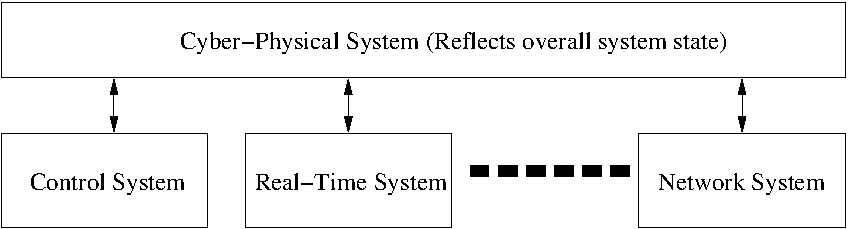
\includegraphics[width=0.45\textwidth]{Figures/cps-n-domains.pdf}
%    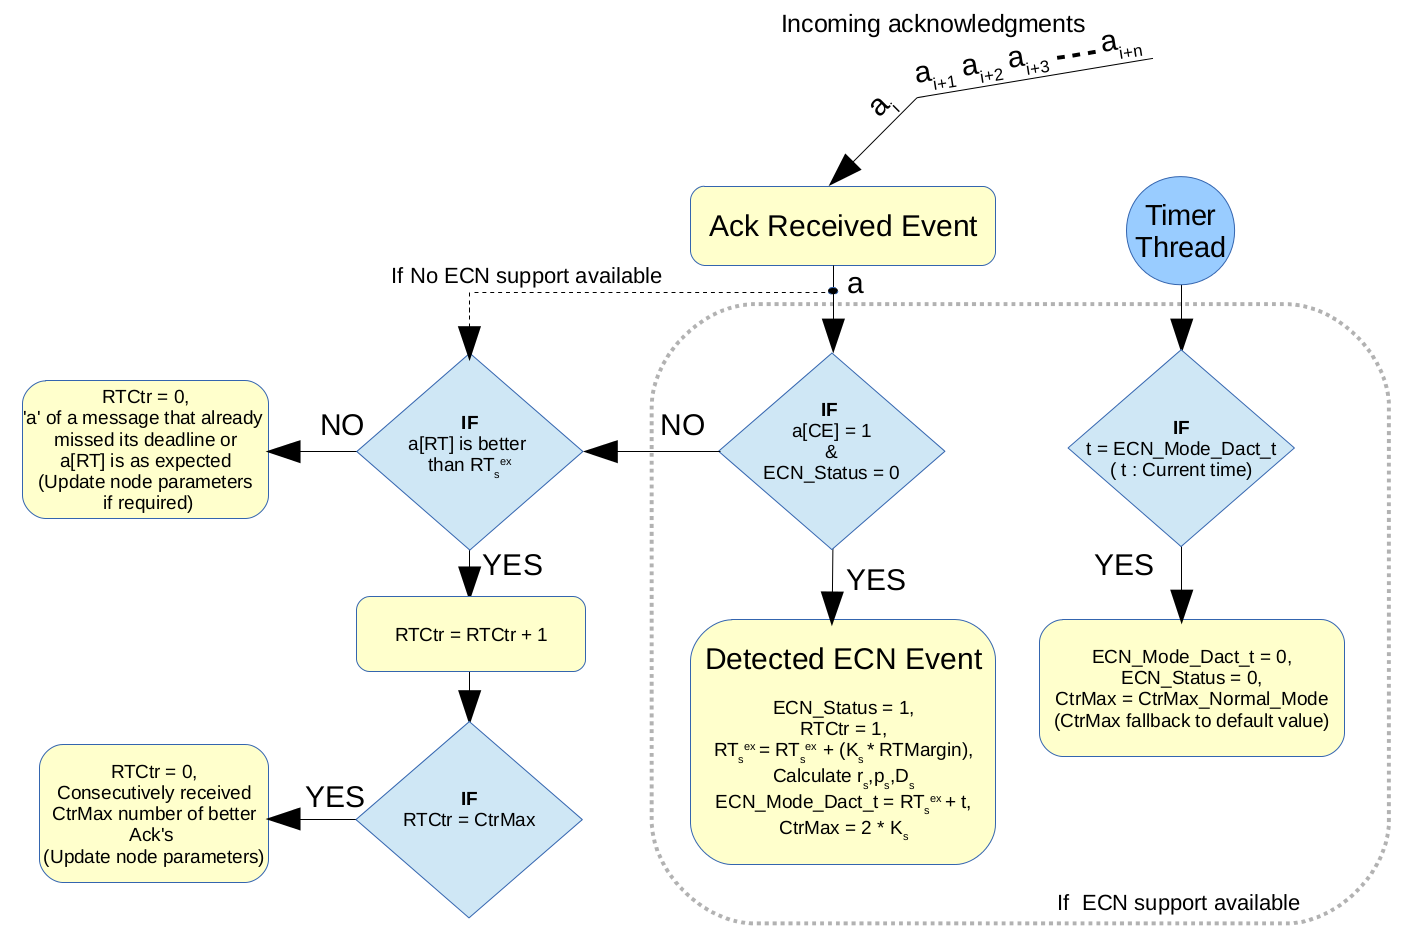
\includegraphics[width=0.9\columnwidth]{Figures/iccps2014/ECN_flow.png}
    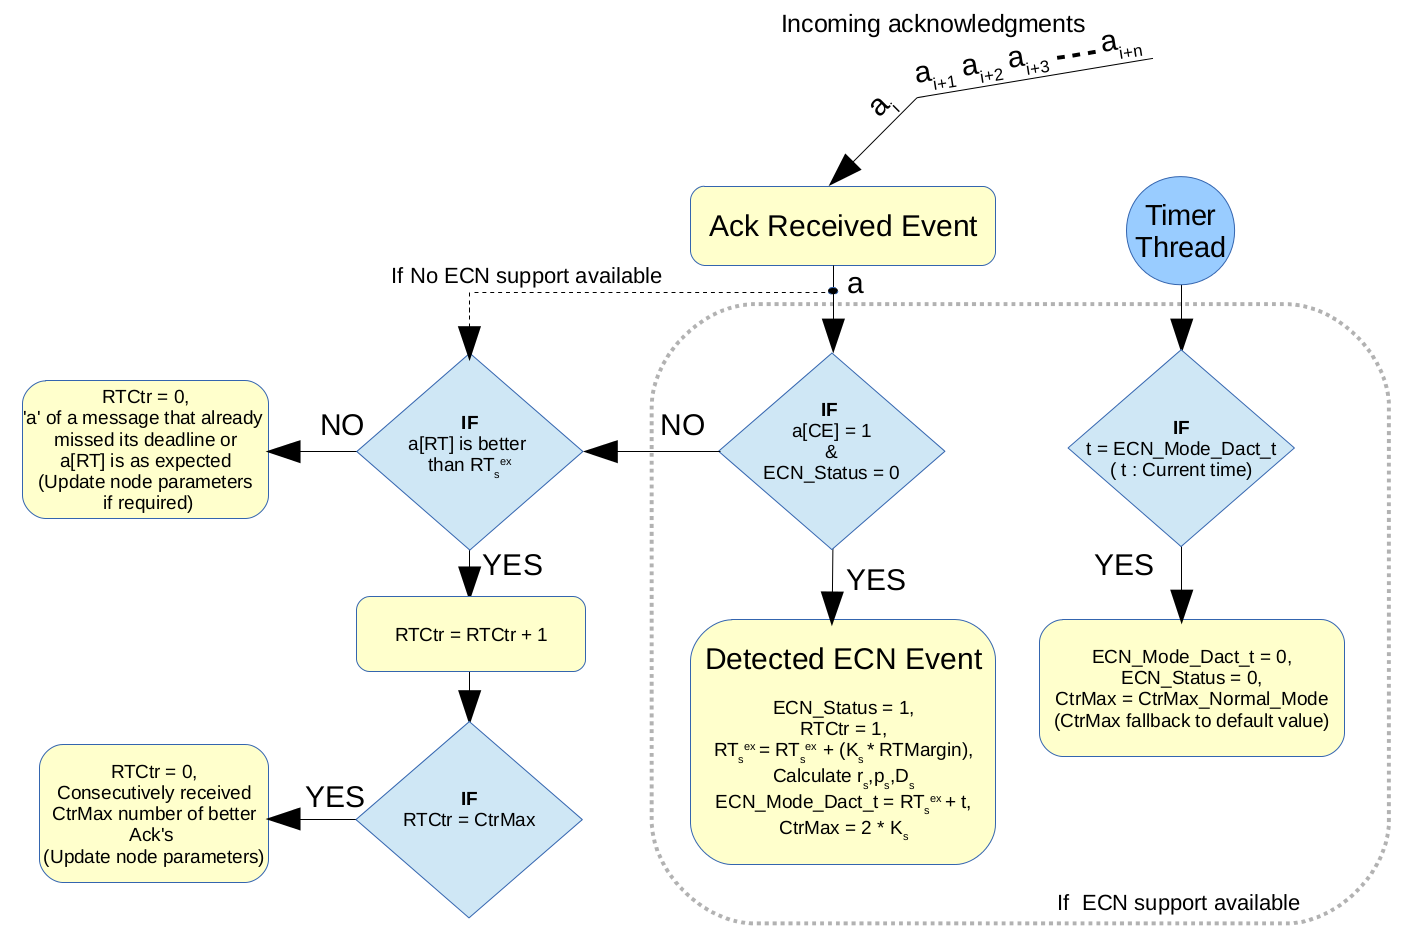
\includegraphics[scale=0.34]{Figures/iccps2014/ECN_flow.png}
  \caption{Flowchart Of $Ack ~Received$ Event With ECN Capable Transport}
  \label{fig:ECN_flow}
  \end{center}
\end{figure*}

{\bf Solution. }To avoid triggering of \textit{Ack received is better} event in ECN mode, we increase the $CtrMax$ limit to $2*K_s$, as shown in Figure.\ref{fig:ECN_flow}, in \textit{Detected ECN} event block. Increasing $CtrMax$ does not completely eliminate the triggering of \textit{Ack received is better} event, but instead makes it more tough to happen. Although $CtrMax$ is a configurable parameter in ECN mode, similar to as in Normal mode, we recommend setting the value of $CtrMax$ proportional to outstanding messages $K_s$. Note that $CtrMax$ is calculated only once per ECN mode switch.

\section{Varying Quantum Of Power ($\delta$)}
\label{sec:vary_delta} 

In previous section, we have successfully integrated a feature of ECN in our adaptive power message scheduling algorithm.
In this section we make changes to the policy of amount of $\delta$ carried by every power transfer message.
The idea is to vary $\delta$ size in proportion to period $p_s$ (or 1/rate, $1/r_s$). But when we talk about 
internet like network, it is non-trivial to bound the rate of transmission. So, each time a message scheduling 
invariant $I_S$ is evaluated, we make an estimate on total amount of power that can be transferred in the  
current power transfer phase $PT$, provided, the current scheduling parameter $r_s$ (rate) does not change.
Based on this estimate, we calculate $\delta$ as in Equation.\ref{eqn:delta_calc}. 

\begin{equation}
\delta = \frac{P_G - P_A}{r_s * (PT_e - RT_s^{ex})} 
\label{eqn:delta_calc}
\end{equation}	

Where, $P_G$ is total power granted to receiver node $r$, $P_A$ is total power acknowledged from node $r$
(node $r$ (receiver node's) stamps total power received in current $PT$ (power transfer phase) in every $ack$), $r_s$ is current rate of power transfer message,
$PT_e$ is absolute end time of current power transfer phase and $RT_s^{ex}$ is current observed response time of
message.

{\bf Problem. }Message scheduling invariant $I_S$ formed by conjunction of sub invariants $I_k$, $I_c$ and $I_p$, will not reflect 
the correct scheduling system state if $\delta$ is allowed to vary. As $I_k$, satisfied if $K_s$<$K_{max_s}$, no more reflects 
the amount of outstanding power in the grid. $K_s$ only reflects the total outstanding messages in the network, because in varying 
$\delta$ scenario, every power transfer message might carry different amount of $\delta$ along them. 

{\bf Solution. }We derive the bounds on $\delta$ as, $\delta_{min}$ and $\delta_{max}$ based on the physical system tolerance
(allowance) [****input from physical system guys that $\delta_{min}$ and $\delta_{max}$ can be provided, ensuring that the 
system stability won't be affected] without compensating for stability. Now in the physical system analysis, in section\ref{sec:invariants},
where we say "$I_{P1}$ ultimately imposes a limit on $\delta * K$", will not hold. Therefore, we modify the term $\delta K$ 
in Equation 3 to $P_T - P_A$ and restate the Equation as in \ref{eqn:grid4_modified}. 

\begin{equation}
\left\{
\begin{matrix}
I_{P1}: (\omega - \omega_0)^2 \left(D\omega + m \right) \\ + (\omega - \omega_0)(kP^2)  > (P_T - P_A)(\omega - \omega_0)
\end{matrix}
\right\}
\label{eqn:grid4_modified}
\end{equation}

Where, $P_T$ is the total power transferred to node $r$ (receiver node) and 
$P_A$ is the total power acknowledged from node $r$. (Note that $P_G$ is total 
power granted, power transfer stops due to the end of $PT$ or $P_G$ = $P_T$ = $P_A$).

We also modify the sub invariant $I_k$ in scheduling invariant $I_S$ as in
Equations \ref{eqn:mod_Ik}-\ref{eqn:mod_Ikn}.

%\begin{equation}
%I_k: I_{kp} \wedge I_{kn} \wedge I_{kd}
%\label{eqn:mod_Ik}
%\end{equation}	

\begin{equation}
I_k: I_{kp} \wedge I_{kn}
\label{eqn:mod_Ik}
\end{equation}	

\begin{equation}
I_{kp}: (\delta_{new} + (P_T - P_A)) < (\delta_{max}*K_{max_s})
\label{eqn:mod_Ikp}
\end{equation}	

\begin{equation}
I_{kn}: K_s < K_{max_s}
\label{eqn:mod_Ikn}
\end{equation}	

%\begin{equation}
%I_{kd}: (\delta_{new} + (P_T - P_A)) < (\delta_{max}*K_{max_s})
%\label{eqn:mod_Ikd}
%\end{equation}	

Where, $\delta_{new}$ is obtained from Equation ~\ref{eqn:delta_calc}.







\section{Experimental Setup}
\label{sec:exp_setup}

We have implemented our algorithm \textit{MsgSchedModule} for adaptive message scheduling with ECN and varying $\delta$ support using C++ in linux environment. Boost portable C++ source libraries~\cite{boost} were used for timing needs in our \textit{MsgSchedModule}. Network was emulated using OMNet++, an open source network simulator ~\cite{omnet, omnetpaper}. OMNet++ is a discrete event simulator that provides an extensible, modular, component-based C++ simulation library. OMNet++ also supports emulation of network in real time instead of just being a simulator~\cite{mayeromnet}. Real-time scheduler class \textit{cRealTimeScheduler()} in OMNet++ was used in our network emulation.
Figure~\ref{fig:dgi_net} shows the network setup used to emulate every power transfer phase. Nodes (denoted as \textit{realPeer50} and \textit{simPeer0} to \textit{simPeer8}), communicate with each other over links and routers (\textit{router0} to \textit{router5}). Nodes are also capable of generating traffic in the network. Note that \textit{MsgSchedModule} is an external module which connects to \textit{realPeer50} through socket to \textit{localhost} at configured \textit{port}. In this paper, we experiment using \textit{realPeer50} as an excess power node. Routers employ first-in-first-out (FIFO) queue with configurable service time $Q_{st}$ for every (total 4 ports) outgoing port. 
Routers being ECN capable, maintain queue average $Q_{avg}$, check $Q_{avg}$ against $Q_{min}$ and $Q_{max}$ thresholds and set congestion experienced (CE) bit in messages if required. Note that $Q_{min}$, $Q_{max}$ and $Q_{st}$ are configurable parameters. 
For the current paper experiments, $Q_{min}$, $Q_{max}$ and $Q_{st}$ are set to 3, 20 and 0.2s (seconds) respectively.
In the current paper, we focus on studying the behavior of our \textit{MsgSchedModule} featured with ECN support and varying $\delta$ support versus non ECN support and constant $\delta$. For a given power transfer phase, the required input data for \textit{realPeer50} as $P_G$ (amount of power granted by \textit{realPeer50} to some node, say \textit{simPeer8}), $K_{max}$, $RT_s^{ex}$, $RTMargin$ and $CtrMax$ (for Normal mode, because in ECN mode $CtrMax$ increases in proportion to outstanding messages $K$) is assumed to be available from state information phase (Figure 3).

{\bf System configuration, }\textit{realPeer50} is excess power node, \textit{simPeer8} is the node demanding $20000~units$ of power and $K_{max_{global}}$ is set to 20. Since there is only one node \textit{realPeer50} with excess power in the experimenting power transfer phase, $K_{max}$ for \textit{realPeer50} is 20, i.e \textit{realPeer50} can have maximum of 20 outstanding power transfer messages in the network. Quantum of power $\delta$ is set to $10$ for experiments with constant $\delta$, whereas $\delta$ is allowed to vary between $10$ to $30$ ($\delta_{min}$, $\delta_{max}$) for experiments with varying $\delta$. Route between \textit{realPeer50} and \textit{simPeer8} is through \textit{router0<->router2<->router4<->router5}. To experiment with traffic, \textit{simPeer7} and \textit{simPeer5} communicate with each other through route \textit{router2<->router4} and generate messages such that
they occupy \textit{50 percent} of total bandwidth. For all the experiments with traffic, traffic is generated from time $t=5000$ to $t=10000$. 

Considering that \textit{realPeer50} granted $20000~units$ of excess power it has to \textit{simPeer8}, \textit{realPeer50} initializes its local variables as, $P_{G(8)}=20000$, $P_{T(8)}=0$ and $P_{A(8)}=0$. In case of constant $\delta$, whenever \textit{realPeer50} wants to transfer $\delta$ amount of power, invariants $I_S$ and $I_P$ are evaluated, if they return $true$, or are satisfied, then only a power transfer message is dispatched to \textit{simPeer8}. Whereas in varying $\delta$ case, before $I_k$ in $I_S$ is evaluated, \textit{MsgSchedModule} calculates $\delta$ size at that instance of time by Equation 13 and if calculated $\delta$ is greater than $\delta_{max}$ then $\delta$ is set equal to $\delta_{max}$ or if calculated $\delta$ is less than $\delta_{min}$ then $\delta$ is set equal to $\delta_{min}$.

\begin{figure}[htb]
  \begin{center}
    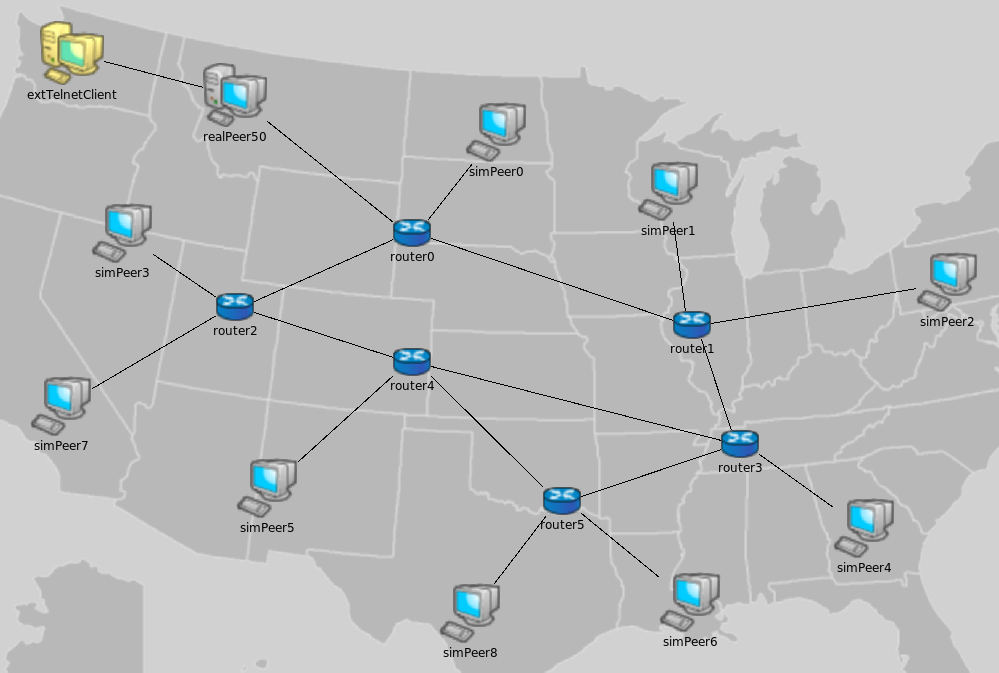
\includegraphics[width=0.50\textwidth]{Figures/iccps2014/dgi_net.png}
  \caption{Emulated Network in OMNet++}
  \label{fig:dgi_net}
  \end{center}
\end{figure}

\subsection{Experimental Results}
\label{sec:exp_results}


%----------------------------------------
\begin{figure}[htb]
  \begin{center}

    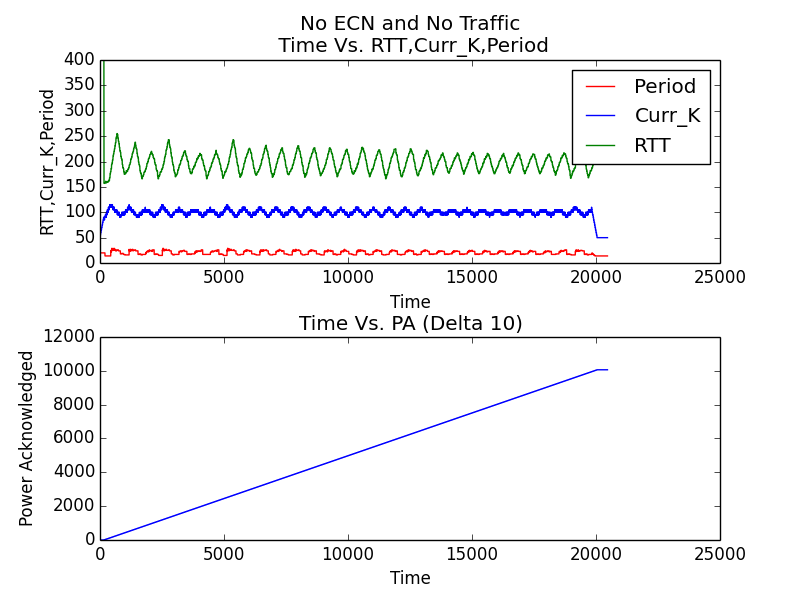
\includegraphics[width=0.50\textwidth]{Figures/iccps2014/no_ecn_no_tr_d10.png}
  \caption{No ECN, No Traffic, $\delta$ = 10}
  \label{fig:no_ecn_no_tr_d10}
    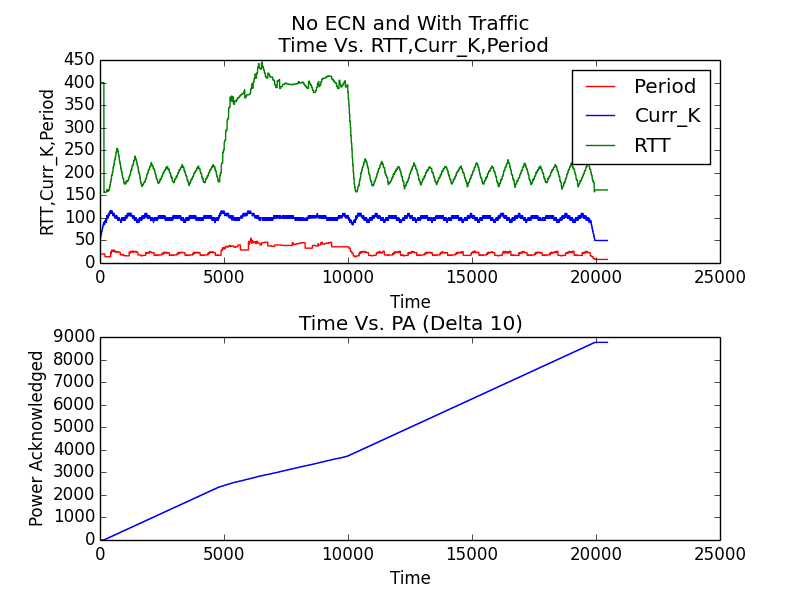
\includegraphics[width=0.50\textwidth]{Figures/iccps2014/no_ecn_w_tr_d10.png}
  \caption{No ECN, With Traffic, $\delta$ = 10}
  \label{fig:no_ecn_w_tr_d10}

  \end{center}
\end{figure}
%----------------------------------------
%----------------------------------------
\begin{figure}[htb]
  \begin{center}

    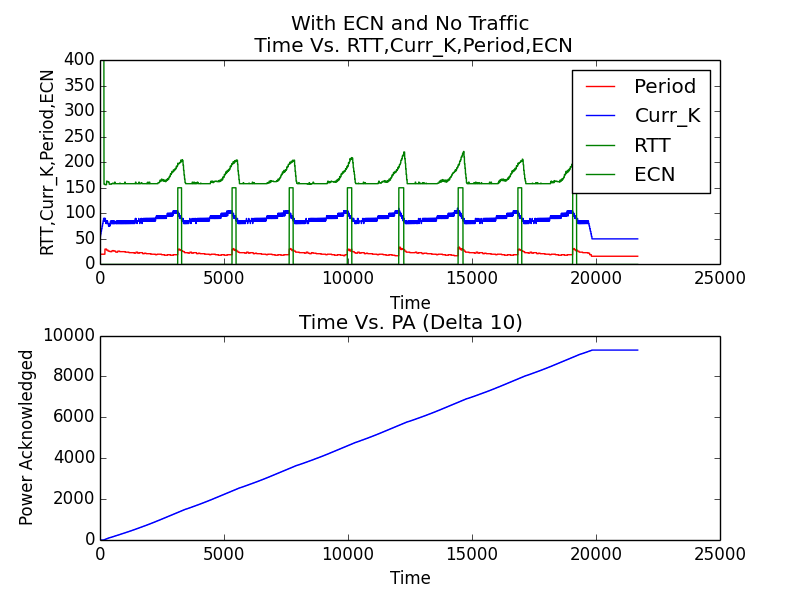
\includegraphics[width=0.50\textwidth]{Figures/iccps2014/w_ecn_no_tr_d10.png}
  \caption{With ECN, No Traffic, $\delta$ = 10}
  \label{fig:w_ecn_no_tr_d10}
    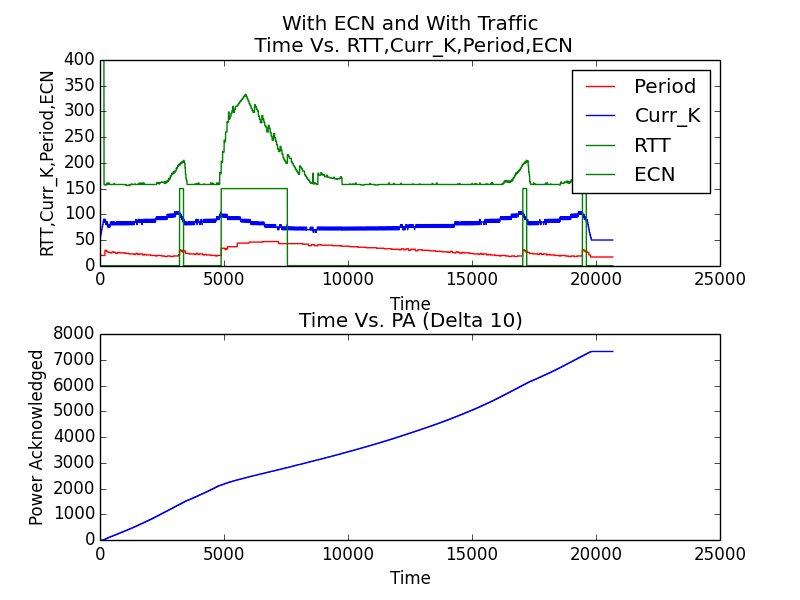
\includegraphics[width=0.50\textwidth]{Figures/iccps2014/w_ecn_w_tr_d10.png}
  \caption{With ECN, With Traffic, $\delta$ = 10}
  \label{fig:w_ecn_w_tr_d10}

  \end{center}
\end{figure}
%----------------------------------------
%----------------------------------------
\begin{figure}[htb]
  \begin{center}
  
    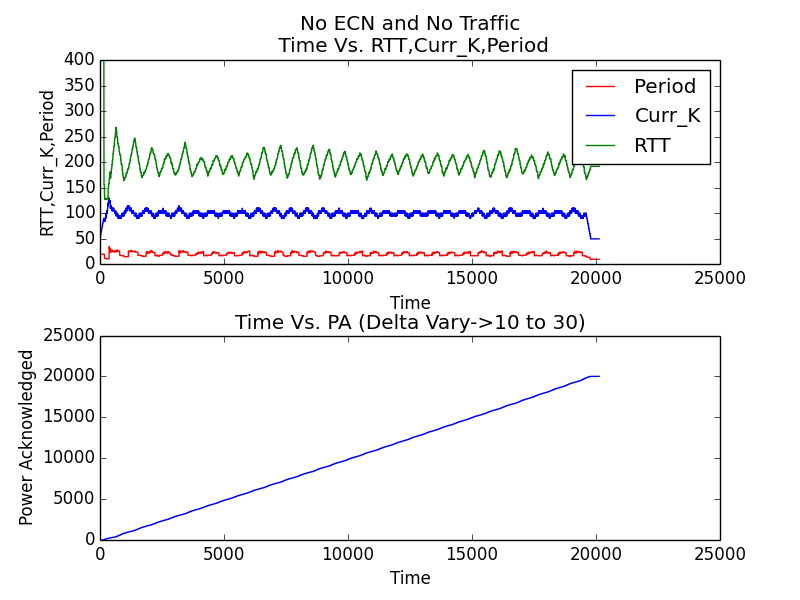
\includegraphics[width=0.50\textwidth]{Figures/iccps2014/no_ecn_no_tr_d10_30.png}
  \caption{No ECN, No Traffic, Vary $\delta$ 10 to 30}
  \label{fig:no_ecn_no_tr_d10_30}
    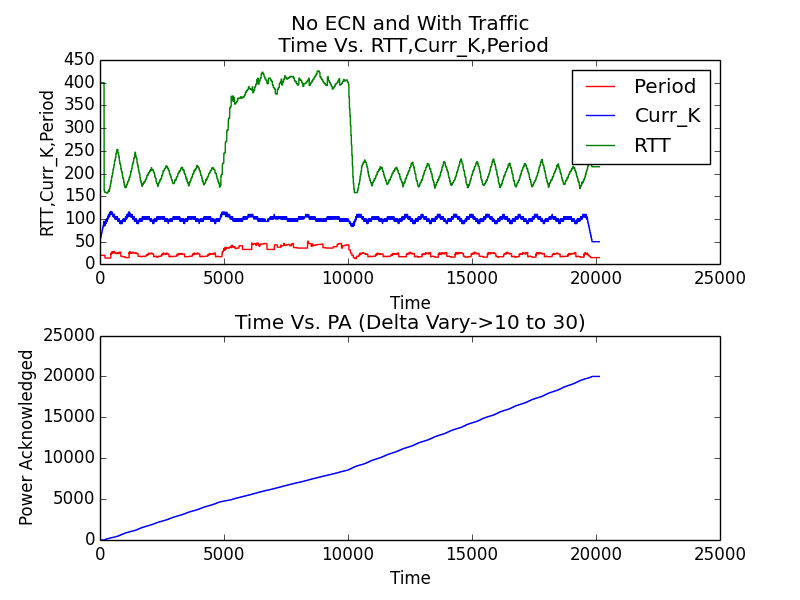
\includegraphics[width=0.50\textwidth]{Figures/iccps2014/no_ecn_w_tr_d10_30.png}
  \caption{No ECN, With Traffic, Vary $\delta$ 10 to 30}
  \label{fig:no_ecn_w_tr_d10_30}

  \end{center}
\end{figure}
%----------------------------------------
%----------------------------------------
\begin{figure}[htb]
  \begin{center}

    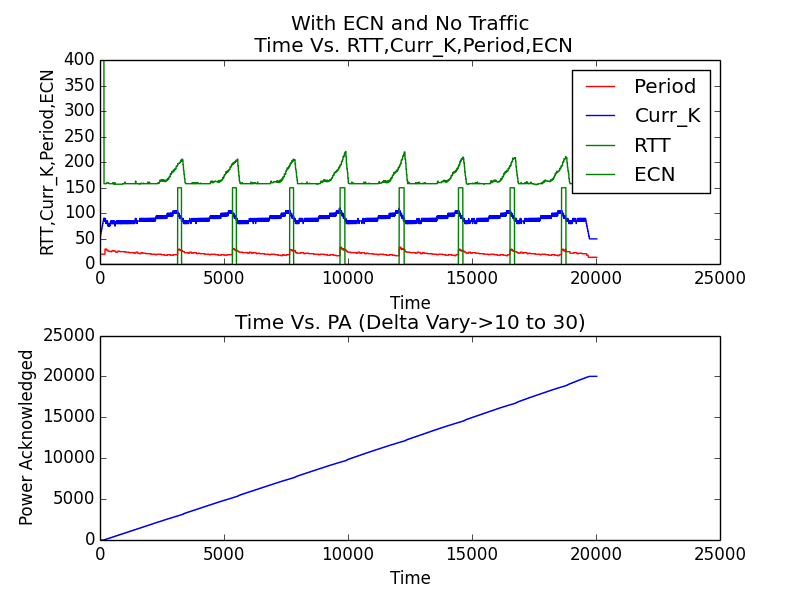
\includegraphics[width=0.50\textwidth]{Figures/iccps2014/w_ecn_no_tr_d10_30.png}
  \caption{With ECN, No Traffic, Vary $\delta$ 10 to 30}
  \label{fig:w_ecn_no_tr_d10_30}
    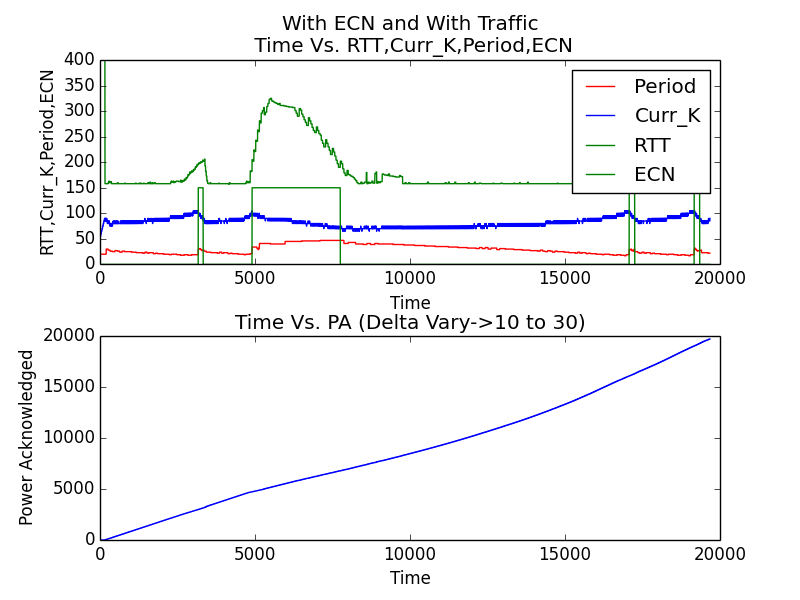
\includegraphics[width=0.50\textwidth]{Figures/iccps2014/w_ecn_w_tr_d10_30.png}
  \caption{With ECN, With Traffic, Vary $\delta$ 10 to 30}
  \label{fig:w_ecn_w_tr_d10_30}

  \end{center}
\end{figure}
%----------------------------------------












\section{Conclusions}
\section*{Acknowledgments}

\bibliographystyle{abbrv}
\bibliography{sigproc}  % sigproc.bib is the name of the Bibliography in this case
% You must have a proper ".bib" file
%  and remember to run:
% latex bibtex latex latex
% to resolve all references

\begin{thebibliography}{10}

\setlength{\itemsep}{-0.01mm}
\footnotesize

\bibitem{cyphy}
{IEEE} workshop on design, modeling and evaluation of cyber physical systems.

\bibitem{omnet}
The {OMNeT}++ discrete event simulation system.

\bibitem{aikat2003variability}
J.~Aikat, J.~Kaur, F.~Smith, and K.~Jeffay.
\newblock Variability in tcp round-trip times.
\newblock In {\em Internet Measurement Conference: Proceedings of the 3 rd ACM
  SIGCOMM conference on Internet measurement}, volume~27, pages 279--284, 2003.

\bibitem{5622003}
R.~Akella, F.~Meng, D.~Ditch, B.~McMillin, and M.~Crow.
\newblock Distributed power balancing for the freedm system.
\newblock In {\em Smart Grid Communications (SmartGridComm), 2010 First IEEE
  International Conference on}, pages 7 --12, October 2010.

\bibitem{alur94}
R.~Alur and D.~L. Dill.
\newblock A theory of timed automata.
\newblock {\em Theoretical Computer Science}, 126(2):183--235, 1994.

\bibitem{Bak2010}
S.~Bak, A.~Greer, and S.~Mitra.
\newblock Hybrid cyberphysical system verification with simplex using discrete
  abstractions.
\newblock In {\em Real-Time and Embedded Technology and Applications Symposium
  (RTAS), 2010 16th IEEE}, pages 143 --152, april 2010.

\bibitem{5587717}
S.~Bensalem, A.~Legay, T.-H. Nguyen, J.~Sifakis, and R.~Yan.
\newblock Incremental invariant generation for compositional design.
\newblock In {\em Theoretical Aspects of Software Engineering (TASE), 2010 4th
  IEEE International Symposium on}, pages 157 --167, aug. 2010.

\bibitem{GarlanKrogh2010}
A.~Bhave, B.~Krogh, D.~Garlan, and B.~Schmerl.
\newblock Multi-domain modeling of cyber-physical systems using architectural
  views.
\newblock In {\em Proceedings of the 1st Analytic Virtual Integration of
  Cyber-Physical Systems Workshop.}, 30 November 2010.
\newblock Co-located with RTSS 2010.

\bibitem{branicky98}
M.~S. Branicky.
\newblock Multiple lyapunov functions and other analysis tools for switched and
  hybrid systems.
\newblock {\em IEEE Transactions on Automatic Control}, 43(4):475--482, 1998.

\bibitem{Buttazzo_IEEE_Jornl_2002}
G.~Buttazzo, G.~Lipari, M.~Caccamo, and L.~Abeni.
\newblock Elastic scheduling for flexible workload management.
\newblock {\em Computers, IEEE Transactions on}, 51(3):289 --302, mar 2002.

\bibitem{chutinan03}
A.~Chutinan and B.~H. Krogh.
\newblock Computational techniques for hybrid system verification.
\newblock {\em IEEE Transactions on Automatic Control}, 48:64--75, January
  2003.

\bibitem{Alfaro}
L.~de~Alfaro and M.~Stoelinga.
\newblock Interfaces: A game-theoretic framework to reason about open systems.
\newblock In {\em FOCLASA 03: Proceedings of the 2nd International Workshop on
  Foundations of Coordination Languages and Software Architectures, Electronic
  Notes on Theoretical Computer Science}. Elsevier Science Publishers, 2003.

\bibitem{DerlerLeeSangiovanniVincentelli12_ModelingCyberPhysicalSystems}
P.~Derler, E.~A. Lee, and A.~Sangiovanni-Vincentelli.
\newblock Modeling cyber-physical systems.
\newblock {\em Proceedings of the IEEE (special issue on CPS)}, 100(1):13 --
  28, January 2012.

\bibitem{AdaptiveScheduling_DASC_1999}
B.~Doerr, T.~Venturella, R.~Jha, C.~Gill, and D.~Schmidt.
\newblock Adaptive scheduling for real-time, embedded information systems.
\newblock In {\em Digital Avionics Systems Conference, 1999. Proceedings.
  18th}, volume 1/17 pp. vol.1, pages 2.D.5--1 --2.D.5--9 vol.1, nov 1999.

\bibitem{donkers11}
M.~C.~F. Donkers, W.~P. M.~H. Heemels, N.~van~de Wouw, and L.~Hetel.
\newblock Stability analysis of networked control systems using a switched
  linear systems approach.
\newblock {\em IEEE Transactions on Automatic Control}, 56:2101--2115, 2011.

\bibitem{floyd1994tcp}
S.~Floyd.
\newblock Tcp and explicit congestion notification.
\newblock {\em ACM SIGCOMM Computer Communication Review}, 24(5):8--23, 1994.

\bibitem{guo2003bayesian}
D.~Guo and X.~Wang.
\newblock Bayesian inference of network loss and delay characteristics with
  applications to tcp performance prediction.
\newblock {\em Signal Processing, IEEE Transactions on}, 51(8):2205--2218,
  2003.

\bibitem{henia_ernst_rtss_2007}
R.~Henia and R.~Ernst.
\newblock Scenario aware analysis for complex event models and distributed
  systems.
\newblock In {\em IEEE Real-Time Systems Symposium}, pages 171--180, Los
  Alamitos, CA, USA, 2007.

\bibitem{henzinger96}
T.~A. Henzinger.
\newblock The theory of hybrid automata.
\newblock In {\em IEEE Symposium on Logic in Computer Science}, pages 278--292,
  1996.

\bibitem{hespanha07}
J.~P. Hespanha, P.~Naghshtabrizi, and Y.~Xu.
\newblock A survey of recent results in networked control systems.
\newblock {\em Proceedings of the IEEE}, 95:138--162, 2007.

\bibitem{Hoare85}
C.~Hoare.
\newblock {\em Communicating Sequential Processes}.
\newblock Prentice Hall, 1985.

\bibitem{hollot2001control}
C.~Hollot, V.~Misra, D.~Towsley, and W.~Gong.
\newblock A control theoretic analysis of red.
\newblock In {\em INFOCOM 2001. Twentieth Annual Joint Conference of the IEEE
  Computer and Communications Societies. Proceedings. IEEE}, volume~3, pages
  1510--1519. IEEE, 2001.

\bibitem{huang11}
A.~Q. Huang, M.~L. Crow, G.~T. Heydt, J.~P. Zheng, and S.~J. Dale.
\newblock {The Future Renewable Electric Energy Delivery and Management
  (FREEDM) System: The energy internet}.
\newblock {\em Proceedings of the IEEE}, 99(1):133--148, Jan. 2011.

\bibitem{jiang2002passive}
H.~Jiang and C.~Dovrolis.
\newblock Passive estimation of tcp round-trip times.
\newblock {\em ACM SIGCOMM Computer Communication Review}, 32(3):75--88, 2002.

\bibitem{SmartGridLoadScheduling}
I.~Koutsopoulos and L.~Tassiulas.
\newblock Control and optimization meet the smart power grid: scheduling of
  power demands for optimal energy management.
\newblock In {\em Proceedings of the 2nd International Conference on
  Energy-Efficient Computing and Networking}, e-Energy '11, pages 41--50, 2011.

\bibitem{DAC_2012_CPS_verification}
P.~Kumar, D.~Goswami, S.~Chakraborty, A.~Annaswamy, K.~Lampka, and L.~Thiele.
\newblock A hybrid approach to cyber-physical systems verification.
\newblock In {\em 49th ACM/EDAC/IEEE Design Automation Conference (DAC)}, pages
  688 --696, june 2012.

\newpage

\bibitem{ReconfigurationCBSECRTST2012}
P.~Kumar, N.~Stoimenov, and L.~Thiele.
\newblock An algorithm for online reconfiguration of resource reservations for
  hard real-time systems.
\newblock In {\em ECRTS}, pages 245--254, 2012.

\bibitem{liberzon03}
D.~Liberzon.
\newblock {\em Switching in Systems and Control}.
\newblock Birkhauser, Boston, 2003.

\bibitem{liu00}
J.~Liu.
\newblock {\em Real-Time Systems}.
\newblock Prentice Hall, 2000.

\bibitem{martin2000analysis}
H.~Martin, A.~McGregor, and J.~Cleary.
\newblock Analysis of internet delay times.
\newblock {\em Measurement}, 2000.

\bibitem{OwickiGries1976}
S.~Owicki and D.~Gries.
\newblock An axiomatic proof technique for parallel programs.
\newblock {\em Acta Informatica}, 6:319--340, 1976.

\bibitem{paul12thesis}
T.~Paul.
\newblock {\em Unified Knowledge Model for Stability Analysis in Cyber Physical
  Systems}.
\newblock Missouri University of Science and Technology, 2012.

\bibitem{paul2011}
T.~Paul, J.~Kimball, M.~Zawodniok, T.~Roth, and B.~McMillin.
\newblock Invariants as a unified knowledge model for cyber-physical systems.
\newblock In {\em Service-Oriented Computing and Applications (SOCA), 2011 IEEE
  International Conference on}, pages 1 --8, dec. 2011.



\bibitem{pei2009passive}
Y.~Pei, H.~Wang, and S.~Cheng.
\newblock A passive method to estimate tcp round trip time from nonsender-side.
\newblock In {\em Computer Science and Information Technology, 2009. ICCSIT
  2009. 2nd IEEE International Conference on}, pages 43--47. IEEE, 2009.



\bibitem{quet2002guidelines}
P.~Quet, S.~Chellappan, A.~Durresi, M.~Sridharan, H.~{\"O}zbay, and R.~Jain.
\newblock Guidelines for optimizing multi-level ecn, using fluid flow based tcp
  model.
\newblock {\em Proc. ITCOM-2002}, pages 106--116, 2002.

%\newpage

\bibitem{ramakrishnan1999proposal}
K.~Ramakrishnan and S.~Floyd.
\newblock A proposal to add explicit congestion notification (ecn) to ip.
\newblock Technical report, RFC 2481, January, 1999.

\bibitem{ramakrishnan2001addition}
K.~Ramakrishnan, S.~Floyd, D.~Black, et~al.
\newblock The addition of explicit congestion notification (ecn) to ip, 2001.

\bibitem{real_crespo_rts_2004}
J.~Real and A.~Crespo.
\newblock Mode change protocols for real-time systems: A survey and a new
  proposal.
\newblock {\em Real-Time Systems}, 26(2):161--197, 2004.

\bibitem{sha_rts_1989}
L.~Sha, R.~Rajkumar, J.~Lehoczky, , and K.~Ramamritham.
\newblock Mode change protocols for priority-driven preemptive scheduling.
\newblock {\em Real-Time Systems}, 1(3):243--264, 1989.

\bibitem{shakkottai2004rtt}
S.~Shakkottai, R.~Srikant, N.~Brownlee, A.~Broido, et~al.
\newblock The rtt distribution of tcp flows in the internet and its impact on
  tcp-based flow control.
\newblock 2004.

\bibitem{DBLP:SitzoffG93}
M.~Sintzoff and F.~Geurts.
\newblock Analysis of dynamical systems using predicate transformers -
  attraction and composition.
\newblock In {\em Analysis of Dynamical and Cognitive Systems}, pages 227--260,
  1993.

\bibitem{stoimenov_date_2009}
N.~Stoimenov, S.~Perathoner, and L.~Thiele.
\newblock Reliable mode changes in real-time systems with fixed priority or edf
  scheduling.
\newblock In {\em Design, Automation and Test in Europe}, pages 99--104. IEEE,
  April 2009.

\bibitem{tomlin03}
C.~J. Tomlin, I.~Mitchell, A.~M. Bayen, and M.~Oishi.
\newblock Computational techniques for the verification of hybrid systems.
\newblock {\em Proceedings of the IEEE}, 91:986--1001, July 2003.

\bibitem{omnetpaper}
A.~Varga.
\newblock The omnet++ discrete event simulation system.
\newblock {\em Proceedings of the European Simulation Multiconference
  (ESM'2001)}, June 2001.

\bibitem{FeedbackScheduling07}
F.~Xia, G.~Tian, and Y.~Sun.
\newblock Feedback scheduling: an event-driven paradigm.
\newblock {\em SIGPLAN Not.}, 42(12):7--14, Dec. 2007.

\bibitem{ye98impulse}
H.~Ye, A.~N. Michel, and L.~Hou.
\newblock Stability analysis of systems with impulse effects.
\newblock {\em IEEE Transactions on Automatic Control}, 43(12):1719--1723,
  1998.

\bibitem{ye98hybrid}
H.~Ye, A.~N. Michel, and L.~Hou.
\newblock Stability theory for hybrid dynamical systems.
\newblock {\em IEEE Transactions on Automatic Control}, 43(4):461--474, 1998.

\bibitem{Zhu:2010:MEE:1795194.1795196}
Y.~Zhu, E.~Westbrook, J.~Inoue, A.~Chapoutot, C.~Salama, M.~Peralta, T.~Martin,
  W.~Taha, M.~O'Malley, R.~Cartwright, A.~Ames, and R.~Bhattacharya.
\newblock Mathematical equations as executable models of mechanical systems.
\newblock In {\em Proceedings of the 1st ACM/IEEE International Conference on
  Cyber-Physical Systems}, ICCPS '10, pages 1--11, New York, NY, USA, 2010.
  ACM.

% new bib for iccps2014

%\bibitem{hadidraft}
%J.~Hadi Salim, B.~Nandy, N.~Seddigh.
%\newblock A Proposal for Backward ECN for the Internet Protocol (IPv4/IPv6).
%\newblock {\em Internet Draft, draftsalim-jhsbnns-ecn-00.txt.}

\bibitem{acsmartgrid}
A.~Choudhari, H.~Ramaprasad, T.~Paul, J.~Kimball, M.~Zawodniok, B.~McMillin, S.~Chellappan.
\newblock Stability of a Cyber-Physical Smart Grid System using Cooperating Invariants.
\newblock In {\em Proceedings of the 37th Annual IEEE International Computer Software and 
Applications Conference}, COMPSAC, Kyoto, Japan, 2013.

\bibitem{Davidebecn}
D.~Bergamasco.
\newblock Datacenter Ethernet Congestion Management: Backward Congestion Notification.
\newblock {\em IEEE 802.1 Meeting, May 2005.}

\bibitem{Davidebecnv2}
D.~Bergamasco, R.~Pan.
\newblock Backward Congestion Notification Version 2.0.
\newblock {\em IEEE 802.1 Meeting, September 2005.}

\bibitem{jiangfecn}
J.~Jiang, R.~Jain, C.~So-In.
\newblock Congestion Management for Ethernet In Datacenter Application Using Forward Explicit Rate Notification.
\newblock {\em WUSTL technical report, 2007.}

\bibitem{jiangefecn}
C.~So-In, R.~Jain, J.~Jiang.
\newblock Enhanced Forward Explicit Congestion Notification (E-FECN) Scheme for Datacenter Ethernet Networks.
\newblock In {\em Proceedings of 2008 International Symposium on Performance Evaluation of Computer and Telecommunication Systems}, 
SPECTS, Edinburgh, UK, June 16-18, 2008.

\bibitem{marekecnstudy}
M.~Malowidzki.
\newblock Simulation-Based Study Of ECN Performance In Red Networks.

\bibitem{boost}
\newblock The boost library.
\newblock {\em http://www.boost.org}


\bibitem{mayeromnet}
C.~P.~Mayer, T.~Gamer.
\newblock Integrating real world applications into OMNeT++.
\newblock {\em Telematics Technical Report, TM-2007-2}, Universit\"{a}t Karlsruhe (TH), Feb. 2008. ISSN 1613-849X.


\end{thebibliography}


%
% ACM needs 'a single self-contained file'!
%
%APPENDICES are optional
%\balancecolumns
\appendix
%Appendix A

Appendix goes here.

% That's all folks!
\end{document}
